



%\section{Proyectos de Investigación}
%\subsection{Visión por Computadora}
\begin{frame}{\citetitle{MarcoNuno_CongArbIng_2014_07_00}}
\begin{block}{} 
\begin{columns}
\begin{column}{0.4\textwidth}
		\begin{itemize}
		\item Detección y conteo de autómoviles 
		\item Videos capturados desde pueden peatonales
		\item  Detectar regiones de movimiento 
		\end{itemize}
\end{column}
\begin{column}{0.6\textwidth}  
    \begin{center}
     %%%%% this is a minipage, so \textwidth is already adjusted to the size of the column
     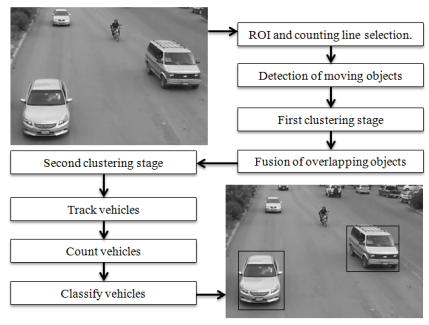
\includegraphics[width=0.70\textwidth]{Figs/TrafficFlow}
     \end{center}
\end{column}
\end{columns}
\end{block} 
%\footnotetext{Raul Humberto Peña-González and Marco Aurelio Nuño-Maganda. \textbf{Computer vision based real-time vehicle tracking and classification system}. In 2014 IEEE 57th International Midwest Symposium on Circuits and Systems (MWSCAS 2014), pages 679–682, Agosto 2014. http://doi.org/10.1109/MWSCAS.2014.6908506ISBN: 978-1-4799-4132-2}
\footnotetext[1]{\fullcite{MarcoNuno_CongArbIng_2014_07_00}}
\setcounter{footnote}{0}


\end{frame}

\begin{frame}{Proyectos de Investigación}
\begin{block}{Seguimiento y Clasificación de Vehículos (2)} 
\begin{columns}
\begin{column}{0.4\textwidth}
		\begin{itemize}
		\item Se capturaron videos de diferentes ubicaciones
		\item Se estimó la densidad de flujo de trafico y por tipo de vehiculo
		\item Idea original: detectar conductores usando telefono celular al manejar
		\end{itemize}
\end{column}
\begin{column}{0.6\textwidth}  
    \begin{center}
     %%%%% this is a minipage, so \textwidth is already adjusted to the size of the column
     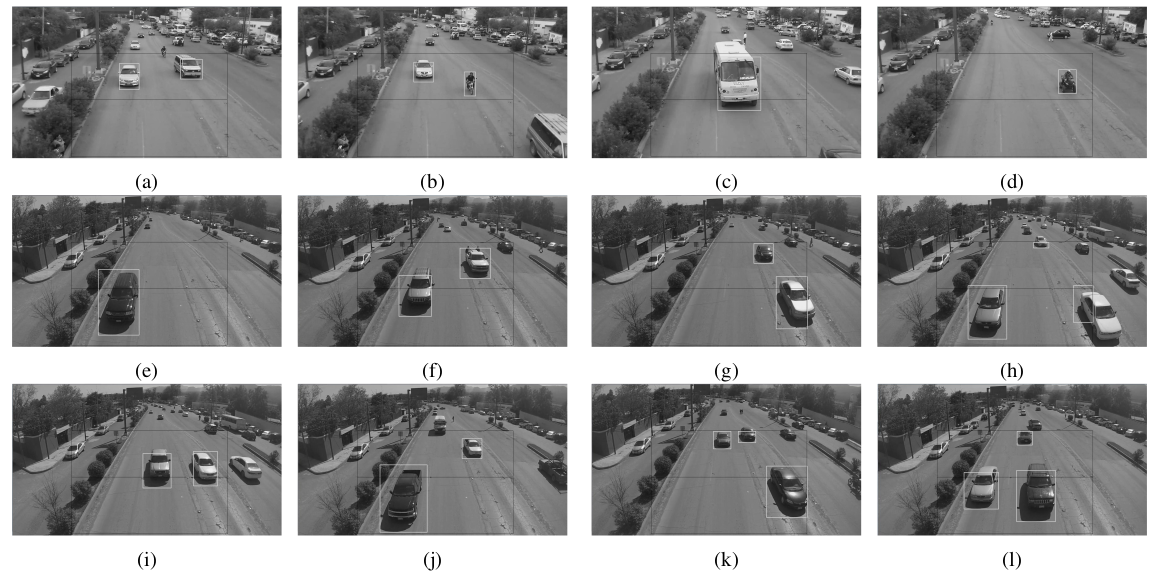
\includegraphics[width=0.8\textwidth]{Figs/TrafficFlow2}
     \end{center}
\end{column}
\end{columns}
\end{block} 
\setcounter{footnote}{0}
\end{frame}





